%==================================================
%CAPITULO II
%=================================================

\chapter{Nociones Básicas de Topología }



\section{Enfoque axiomático de las  estructuras métricas} 
\marginnote{\vspace{-2cm}
\begin{center}
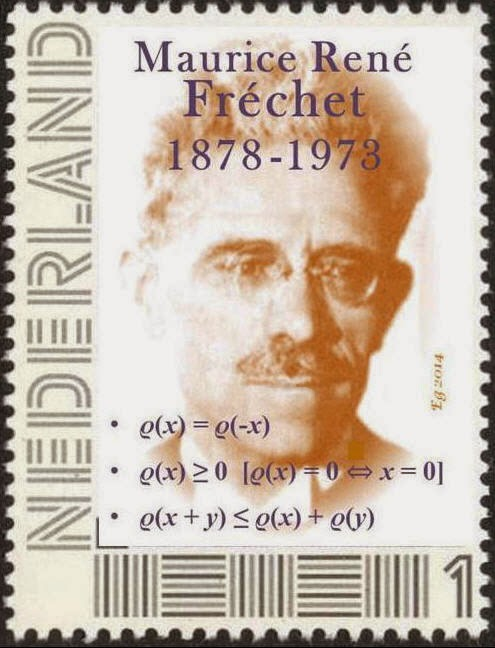
\includegraphics[scale=.2]{imagenes/Frechet.jpg}
\end{center}
\small
Maurice René Fréchet; (Maligny, 2 de septiembre de 1878 - París, 4 de junio de 1973) fue un matemático francés. Trabajó en topología, teoría de la probabilidad y la estadística. 
Sus trabajos en análisis funcional lo empujaron a buscar un marco más general que el espacio euclídeo introduciendo la noción de espacio métrico\index[personas]{Frechet}. 
}
Uno de los conceptos fundamentales de la matemática es la noción de \index{Distancia}\emph{distancia}. Esta noción está presente en multitud de actividades humanas, desde el comercio a la descripción del cosmos. En matemática medimos distancias en el plano y en el espacio y en las representaciones algebraicas de ellos  $\rr^2$ y $\rr^3$. Más generalmente  en espacios euclideanos $n$-dimensionales $\rr^n$. Desde comienzos del siglo XX los matemáticos fueron extendiendo la noción de distancia a conjuntos compuestos de los más diversos entes, matrices, funciones, funciones que actúan sobre funciones, etc. Esta ubicuidad y multiplicidad del concepto de distancia justifica un tratamiento axiomático de él.








\begin{definicion} Sea $X$ un conjunto y $d:X\times X\rightarrow
\mathbb{R}$ una función. Diremos que $d$ es una \index{Métrica}\emph{métrica} o \emph{distancia}
sobre $X$ si satisface las siguientes propiedades:
	  \begin{itemize}
		   \item[i)]$\forall x \forall y: d(x,y)=0\Leftrightarrow x=y$.
		   \item[ii)] $\forall x \forall y : d(x,y)=d(y,x)$.
		   \item[iii)]$\forall x \forall y \forall z: d(x,z)\leq
				d(x,y)+d(x,z)$.
	  \end{itemize}
Si $d$ es una métrica sobre $X$ diremos, entonces, que el par
$(X,d)$ es un \index{Espacio métrico}\emph{espacio métrico}.
\end{definicion}
\marginnote{
\begin{center}
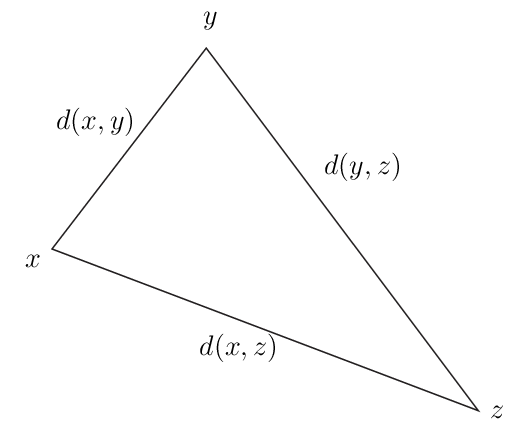
\includegraphics[scale=.25]{imagenes/triag.png}
Desigualdad triangular
\end{center}
}
La desigualdad iii) en la definición anterior se denomina\index{desigualdad triágular}
\emph{desigualdad triágular}, esto debido a que se la puede
pensar como la relación entre un lado de un triágulo y la suma
de los otros dos, ver figura  en el margen.




Veamos ahora algunos ejemplos de espacios métricos.

\begin{ejemplo} La función módulo $|.|:\mathbb{R}\rightarrow
\mathbb{R}$ induce una métrica sobre $\mathbb{R}$, a saber: para
$x,y\in\mathbb{R}$ definimos
\begin{equation}\label{distmod}
	d(x,y)=|x-y|.
\end{equation}
\end{ejemplo}

\begin{ejemplo}\label{ejem,disteuclidea} Sobre $\mathbb{R}^n$
consideremos la función
distancia $d$ definida por
\begin{equation}\label{meteuclidea}
	d(\mathbf{x},\mathbf{y}):=\sqrt{\sum\limits_{i=1}^{n}(x_i-y_i)^2},
\end{equation}
donde $\mathbf{x}=(x_1,\dots,x_n)$ e $\mathbf{y}=(y_1,\dots,y_n)$.
Dejamos al alumno la demostración de que $d$ es una métrica,
ver Ejercicio \vref{ejmeteuclidea}. Esta métrica es conocida
como \emph{métrica euclidea}\index{métrica euclidea} y es la métrica usual que estamos
habituados a considerar.
\end{ejemplo}



\begin{ejemplo} Dado cualquier conjunto no vacío $X$, la
función definida por:
\[
	d(x,y):=\left\{
\begin{array}{ll}
	1, & \hbox{si $x\neq y$;} \\
	0, & \hbox{si $x=y$.} \\
\end{array}
\right.
\]
es una métrica. Esta métrica se denomina \emph{métrica
discreta}.\index{métrica
discreta}
\end{ejemplo}

\begin{ejemplo}\label{ejem,distsobrecont} Dado un conjunto $X$,
definamos $\mathcal{A}(X)$
como el conjunto de todas las funciones acotadas $f:X\rightarrow
\mathbb{R}$. Entonces $(\mathcal{A}(X),d)$ es una métrica,
donde:
\begin{equation}\label{convunifmet}
	d(f,g):=\sup\limits_{x\in X}|f(x)-g(x)|.
\end{equation}
\end{ejemplo}

\begin{ejemplo}\label{ejem,distsobrecontl1} Sea $\mathcal{C}([0,1])$
el conjunto de funciones
continuas $f:[0,1]\rightarrow\mathbb{R}$. Entonces\linebreak
$(\mathcal{C}([0,1]),d)$ es un espacio métrico, donde:
\begin{equation}\label{l1metint}
	d(f,g):=\int_0^1|f(x)-g(x)|dx.
\end{equation}
\end{ejemplo}
\section{Bolas, esferas y diámetro}
Definido lo que es una métrica y un espacio métrico, pasamos a
definir algunas entidades de carácter geométrico, esta son el
concepto de \emph{bola}, \emph{esfera} y \emph{diámetro}.\index{bola} \index{esfera}  \index{diámetro}

\begin{definicion} Sea $(X,d)$ un espacio métrico, $x\in X$ y
$r>0$.
\begin{itemize}
\item[a)]Definimos la bola abierta $B(x,r)$, con centro en $x$ y radio
$r$, por:
\[B(x,r):=\{y\in X:d(x,y)<r\}.\]
\item[b)]Definimos la esfera $E(x,r)$, con centro en $x$ y radio
$r$, por:
\[E(x,r):=\{y\in X:d(x,y)=r\}.\]
\end{itemize}
\end{definicion}

Todos tenemos una concepción de lo que entendemos por una bola,
quizas se nos venga a la mente, y de hecho es un ejemplo, un
círculo en $\mathbb{R}^2$. No obstante, debemos proceder con
cuidado. Estamos considerando métricas generales, ocurrirá que
en algunos espacios métricos las  bolas no se parecen a lo
que comunmente entendemos por este concepto. Esto es debido a que
en nuestra vida cotidiana estamos habituados a considerar la
métrica euclidea, pero en este curso trabajaremos con métricas
muy generales.

En $\mathbb{R}$, con la métrica dada por el módulo, la bola
centrada en $x\in\mathbb{R}$ y radio $r$, no es mas que el
intervalo $(x-r,x+r)$. En la figura \vref{ejembolas}  mostramos
varios ejemplos de bolas en diferentes métricas sobre
$\mathbb{R}^2$, las demostraciones las desarrollaremos en la
clase.


Todavía mas curiosas son las bolas respecto a la métrica
discreta. Sea $(X,d)$ un espacio métrico discreto y $x\in X$,
entonces:

\[B(x,r)=\left\{
\begin{array}{ll}
	\{x\}, & \hbox{si $r<1$;} \\
	X, & \hbox{si $r\geq 1$.} \\
\end{array}
\right.
\]

La esfera la podemos pensar como el borde de la bola, que no
está incluida en la bola abierta. También tenemos en este caso
situaciones que, en un primer momento, nos pueden parecer
extra\~nas. Como casi siempre, el mayor ``grado de
extra\~namiento'' se consigue con la métrica discreta. En este
caso, si $(X,d)$ es un espacio métrico discreto, tenemos:
\[E(x,r)=\left\{
\begin{array}{ll}
	\{x\}, & \hbox{si $r=0$;} \\
	X-\{x\}, & \hbox{si $r=1$;} \\
	\emptyset, & \hbox{si $r\neq 0$ y $r\neq 1$.} \\
\end{array}
\right.
\]

Pasamos a definir, ahora, el concepto de diámetro de un
conjunto.

\begin{definicion} Sea $(X,d)$ un espacio métrico y $A\subset
X$. Definimos el diámetro del conjunto $A$ por:
\[
	\delta(A):=\sup\limits_{x,y\in A}d(x,y).
\]
Eventualmente, podría ocurrir que $\delta(A)=+\infty$.
\end{definicion}
La figura \vref{diamconj} explica, por si sola, el significado del
concepto de diámetro.




\begin{definicion} Un conjunto no vacío $A$ se dirá acotado si
$\delta(A)<\infty$.
\end{definicion}
Es oportuno aclarar que el concepto de acotación depende del
conjunto en si mismo y de la métrica. Así puede ocurrir que
un mismo conjunto sea acotado con una métrica y con otra no.

\begin{ejemplo} En el espacio $\mathbb{R}$, con la métrica del
módulo, el conjunto $(0,+\infty)$ es no acotado. En cambio, con
la métrica discreta todo conjunto, y en particular el dado, lo
es.
\end{ejemplo}

También definiremos la distancia de un punto a un conjunto dado.

\begin{definicion} En un espacio métrico $(X,d)$ se define la
distancia de $x\in X$ a $A\subset X$ como
\[d(x,A):=\inf\limits_{y\in A}d(x,y).\]
\end{definicion}

Demostremos que
\[\delta(B(x,r))\leq 2r.\]
Efectivamente, dados $z$ e $y$ en la bola $B(x,r)$, tenemos, por
la desigualdad triangular
\[d(y,z)\leq d(y,x)+d(x,z)\leq 2r.\]
Tomando supremo sobre $z$ e $y$ obtenemos la afirmación. Notar
que ya no es cierto que $\delta(B(x,r))=2r$. En efecto, por
ejemplo si $(X,d)$ es un espacio métrico discreto, entonces
$\delta(B(x,1/2))=0$.

Ahora probaremos que la unión de conjuntos acostados es, a la
vez, un conjunto acotado.

\begin{proposicion} Sean $(X,d)$ un espacio métrico, $A$ y $B$
subconjuntos acotados de $X$. Entonces $A\cup B$ es acotado.
\end{proposicion}
\begin{demo}  Tenemos que probar que:
	\[\delta(A\cup B)<\infty.\]
Para esto, es suficiente demostrar que $\forall x,y\in A\cup B$
existe una constante $M$, independiente de $x$ e $y$, tal que:
\[d(x,y)\leq M.\]
Sean $z\in A$ y $w\in B$ dos cualesquiera puntos en los conjuntos
indicados. A travez de esta demostración estos puntos estaran
fijos, no importandonos que puntos sean, cualquiera conduce al
mismo argumento. Tomemos, ahora, $x,y\in A\cup B$ cualesquiera,
pero ya no estaran fijos. Si ocurriera que $x$ e $y$ estuvieran
simultaneamente en uno mismo de los conjuntos, supongamos $A$,
entonces tenemos que:
\[d(x,y)\leq \delta(A),\]
de modo que, en este caso, existe una constante $M$ con la
propiedad deseada. Debemos considerar el caso en que $x$ e $y$
esten en ``conjuntos diferentes'', digamos $x\in A$ e $y\in B$.
Entonces tenemos:
\[
	d(x,y)\leq d(x,z)+d(z,w)+d(w,y)\leq \delta(A)+d(z,w)+\delta(B).
\]
El miembro derecho, de la desigualdad anterior, es independiente
de $x$ e $y$, de modo que quedó demostrada la  proposición.
\end{demo}

\section{Conjuntos abiertos} Uno de los conceptos
más importantes, sino el más, de la Topología es el de
conjunto abierto.
\begin{definicion} Sea $(X,d)$ un e.m\footnote{Abreviación para espacio
métrico}. Diremos que $A\subset X$ es un conjunto abierto si
$\forall x\in A\exists r>0$ tal que:
\[
	B(x,r)\subset X.
\]
\end{definicion}
\marginnote{
\begin{center}
	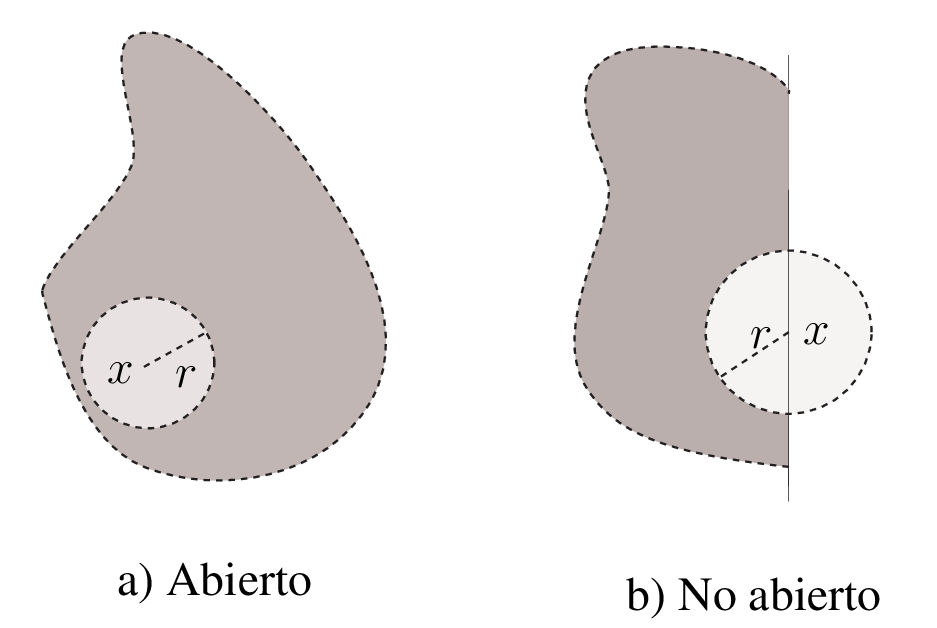
\includegraphics[scale=.15]{imagenes/conjabi.png}
	Conjuntos abiertos y no abiertos.
\end{center}
}
En la figura \vref{conjabi} podemos ver un ejemplo de conjunto
abierto, en $\mathbb{R}^2$ con la métrica euclidea, y otro que
no lo es. La diferencia es que en el conjunto b) el borde (en la
parte recta del conjunto) forma parte del mismo conjunto, entonces
si $x$ está en este borde, toda bola centrada en $x$ contiene
puntos fuera del conjunto.


Un ejemplo, esperable, de conjunto abierto lo constituyen las
bolas abiertas.
\begin{proposicion} Toda bola abierta es un conjunto abierto.
\end{proposicion}
\begin{demo} 
\marginnote{
\begin{center}
	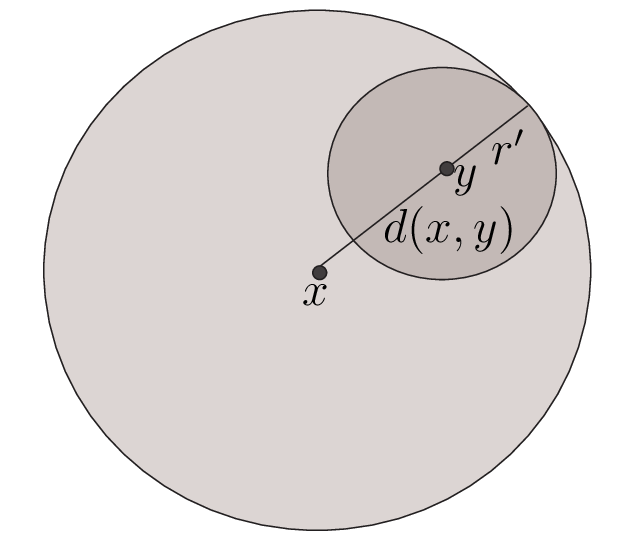
\includegraphics[scale=.18]{imagenes/grafbol.png}\\
	Construcción de $r'$.
\end{center}
}
Sea $x\in X$ y $r>0$. Consideremos la bola abierta
$B(x,r)$. Para demostrar que la bola es abierta, hay que
encontrar, para todo $y\in B(x,r)$, un $r'>0$ tal que
\begin{equation}\label{inclusion}
	B(y,r')\subset B(x,r).
\end{equation}
Sea, pues, $y\in B(x,r)$. Tomemos:
\[r':=r-d(x,y).\]
Ver la figura \vref{construccionrprima} para un gráfico de la
situación. Este $r'$ es mayor que cero. En efecto, como $y$
está en la bola, tenemos que $d(x,y)<r$.




Ahora, veamos la inclusión \vref{inclusion}. Sea $z\in B(y,r')$,
entonces tenemos, por la desigualdad triangular, que:
\[d(x,z)\leq d(x,y)+d(y,z)< d(x,y)+r'<r.\]
Así $z\in B(x,r)$, que es lo que queríamos demostrar.
\end{demo}

Ahora damos dos propiedades de conjuntos abiertos que tendrán
mucha trascendencia más adelante.
\begin{teorema}\label{teo,uniointerabiertos} Sea $I$ un conjunto de índices y
$\{A_i\}_{i\in I}$ una familia de conjuntos abiertos. Entonces:
\begin{itemize}
\item[a)] La unión $\bigcup_{i\in I}A_i$ es un conjunto abierto.
\item[b)] Si $I$ es finito, la intersección $\bigcap_{i\in
I}A_i$ es un conjunto abierto.
\end{itemize}
\end{teorema}
\begin{demo} Empecemos por la propiedad a). Sea $x$ un punto en la
unión, es decir existe algún índice $i_0$ tal que $x\in
A_{i_0}$. Como este $A_{i_0}$ es un conjunto abierto, deberá
existir $r>0$ tal que $B(x,r)\subset A_{i_0}$. Claramente la bola
$B(x,r)$, al ser un subconjunto de $A_{i_0}$ es un subconjunto de
la unión de todos los $A_i$, que es lo que teníamos que
probar.

Ahora veamos b). Podemos suponer que, para algún $n\in
\mathbb{N}$, tenemos que $I=\{1,\dots,n\}$. Sea $x$ un punto en la
intersección. En este caso, $x\in A_i$, para todo $i$. Como cada
$A_i$ es abierto, existen radios $r_i$ tales que $B(x,r_i)\subset
A_i$. Definamos:
\[
	r:=\min\{r_1,\dots,r_n\}.
\]
El mínimo existe, y es mayor que cero, pues hay una cantidad
finita de radios. Ahora tenemos que, como $r\leq r_i$,
$B(x,r)\subset B(x,r_i)\subset A_i$, para todo $i\in I$. Por
consiguiente $B(x,r)$ es un subconjunto de la intersección de
todos los $A_i$.
\end{demo}

Es interesante notar que, en un e.m. discreto $(X,d)$, todo
subconjunto $A\subset X$ es abierto. Efectivamente, en un e.m.
discreto $B(x,1/2)=\{x\}$ para todo $x\in X$. En particular, si
$x\in A$ entonces $B(x,1/2)\subset A$.

\section{Interior de un conjunto y entornos} Como es costumbre,
empezamos con una definición.
\begin{definicion} Sea $(X,d)$ un e.m. y $A\subset X$. Definimos
el interior de $A$, denotaremos este conjunto $A^0$, como el
conjunto de todos los puntos $x\in A$ tales que existe un $r>0$
que satisface $B(x,r)\subset A$.
\end{definicion}

Hay una gran similitud de esta definición con la de conjunto
abierto. De hecho se tiene que un conjunto $A$ es abierto si y
solo si $A=A^0$.

En $\mathbb{R}^2$ con la métrica euclidea podemos visualizar el
interior de un conjunto como la parte del conjunto que no está
sobre el borde de él, ver figura \vref{interiordeconj}.

\begin{figure}
\begin{center}
	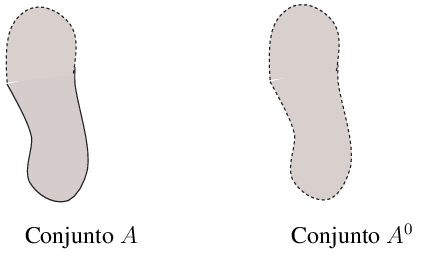
\includegraphics[scale=.5]{imagenes/interio.png}
	\caption{Interior de un conjunto}\label{interiordeconj}
\end{center}
\end{figure}

Tenemos una caracterización alternativa del interior de un
conjunto.

\begin{teorema}\label{teo,mayorabierto} El interior de un conjunto $A$, es el mayor abierto
contenido en $A$.
\end{teorema}
\begin{demo} El hecho de que $A^0$ es abierto y está contenido
en $A$, es consecuencia inmediata de la definición y lo dejamos
como ejercicio. Vamos a demostrar que es el mayor de los abiertos
contenido en $A$. Vale decir, hay que demostrar que si $B$ es un
abierto contenido en $A$, entonces $B\subset A^0$. Sea pues $B$
abierto y $B\subset A$. Tomemos $x\in B$. Como $B$ es abierto
existe un $r>0$ tal que $B(x,r)\subset B\subset A$. Así,
necesariamente $x\in A^0$. Lo que demuestra que $B\subset A^0$.
\end{demo}

Daremos algunas propiedades de la operación de tomar el interior
de un conjunto.
\begin{teorema} Sea $(X,d)$ un e.m., $A$ y $B$ subconjuntos de
$X$.
\begin{itemize}
\item[a)] $(A^0)^0=A^0$
\item[b)] Si $A\subset B$ entonces $A^0\subset B^0$.
\item[c)] $(A\cap B)^0=A^0\cap B^0$.
\end{itemize}
\end{teorema}
\begin{demo} a) Como dijimos, $A^0$ es abierto, por ende
$(A^0)^0=A^0$.

b)$A^0$ es un abierto y además está contenido en $B$, por
consiguiente $A^0\subset B^0$.

c) Como $A\cap B\subset A$ tenemos que, a acausa de b), $(A\cap
B)^0\subset A^0$. De la misma manera $(A\cap B)^0\subset B^0$. Por
consiguiente $(A\cap B)^0\subset A^0\cap B^0$. Para la otra
inclusión, tener en cuenta que $A^0\cap B^0$ es un abierto
contenido en $A\cap B$, por lo tanto $A^0\cap B^0\subset (A\cap
B)^0$.
\end{demo}
 Introducimos otro concepto.

\begin{definicion} En un e.m. el exterior de un conjunto $A$ es el
interior de su complemento. En símbolos ponemos
$\text{Ext}(A)=(A^c)^0$.
\end{definicion}


\begin{definicion} Sea $(X,d)$ un e.m. y $x\in X$. Diremos que $V$
es un entorno de $x$ si $x\in V^0$. También denotaremos por
$E(x)$ al conjunto de todos los entornos de $x$.
\end{definicion}

El anterior es otro de los conceptos claves de la topología.
Observemos que un conjunto abierto es entorno de cada uno de sus
puntos. La recíproca es también cierta, es decir si un
conjunto es entorno de cada uno de sus puntos entonces es abierto.

\begin{proposicion} La intersección de una cantidad finita de
entornos de un punto $x$ en un e.m. $(X,d)$ es, a su vez, un
entorno de $x$.
\end{proposicion}
\begin{demo} Sean $V_i$, $i=1,...,n$, entornos de $x\in X$. Por
definición $x\in V_i^0$ para todo $i=1,...,n$. Entonces $x\in
V_1^0\cap\dots\cap V_n^0=(V_1\cap\dots\cap V_n)^0$. De modo que
$V_1\cap\dots\cap V_n$ es un entorno de $x$. Así queda
establecida la propiedad que expresa la proposición.
\end{demo}

\section{Conjuntos cerrados y clausura de
conjuntos}

Ahora introduciremos el concepto de conjunto cerrado.
\begin{definicion} Un conjunto es cerrado si su complemento es
abierto.
\end{definicion}

Esta sencilla definición hace las nociones de conjunto cerrado y
abierto duales\footnote{Dos tipos de conceptos son duales cuando
cualquier afirmación sobre uno de ellos se convierte en una
afirmación sobre el otro. En este proceso de ``transformación
de enunciados'' hay que traducir cada concepto por su dual. Por
ejemplo, en el caso que nos ocupa, un conjunto cerrado muta en
abierto y las intersecciones mutan en uniones y viceverza. Uniones
e intersecciones son duales como consecuencia de las leyes de de
Morgan}, así veremos que cada propiedad de conjuntos abiertos
induce una correspondiente propiedad sobre conjuntos cerrados.
Tener en cuenta esto en la siguiente teorema.

\begin{teorema}\label{teo,uniointercerrados} Sea $I$ un conjunto de índices y
$\{F_i\}_{i\in I}$ una familia de conjuntos cerrados. Entonces:
\begin{itemize}
\item[a)] La intersección $\bigcap_{i\in I}F_i$ es un conjunto cerrado.
\item[b)] Si $I$ es finito, la unión $\bigcup_{i\in
I}F_i$ es un conjunto cerrado.
\end{itemize}
\end{teorema}
\begin{demo} La afirmaciones a) y b) de este teorema son duales de
las a) y b) del Teorema \vref{teo,uniointerabiertos}. Por ejemplo,
para demostrar a), observemos que, por definición, la siguiente
es una familia de conjuntos abiertos: $\{F_i^c\}_{i\in I}$. De
modo que por a) del Teorema \vref{teo,uniointerabiertos} tenemos
que:
\[\bigcup\limits_{i\in I}F_i^c\]
es un conjunto abierto. De allí que el complemento de este
conjunto es cerrado. Pero el complemento de este conjunto es, en
virtud de las leyes de de Morgan, la intersección de todos los
$F_i$. La propiedad b) se obtiene de la misma manera.
\end{demo}

Ejemplos de conjuntos cerrados son los intervalos cerrados de
$\mathbb{R}$, con la métrica del módulo; las bolas cerradas en
cualquier e.m., es decir los conjuntos de la forma:
\[B'(x,r):=\{y\in X: d(x,y)\leq r\}.\]
Las esferas también resultan ser conjuntos cerrados. Por otra
parte, como en un e.m. discreto todo conjunto es abierto, todo
conjunto, también, es cerrado. La demostración de que los
anteriores son conjuntos cerrados las dejamos como ejercicios. A
lo largo de esta materia veremos varios ejemplos mas de conjuntos
cerrados, encomendamos al estudiante prestar atención a ellos,
puesto que tan importante como aprender las definiciones y
propiedades de determinado concepto, es conocer, y poder construir
ejemplos de ese concepto.

El concepto de interior de un conjunto tiene su dual
correspondiente.
\begin{definicion} Sea $(X,d)$ un e.m.. La clausura de un conjunto $A\subset
X$ se define y denota como se ve a continuación:
\[\C{A}:=(\text{Ext}(A))^c=\bigl[(A^c)^0\bigr]^c.\]
\end{definicion}

 En $\rr^2$ con la métrica euclidea podemos visualizar la
clausura de un conjunto  como el conjunto más su ``borde'', ver
la figura \vref{fig,clausura}.

\begin{figure}
\begin{center}
	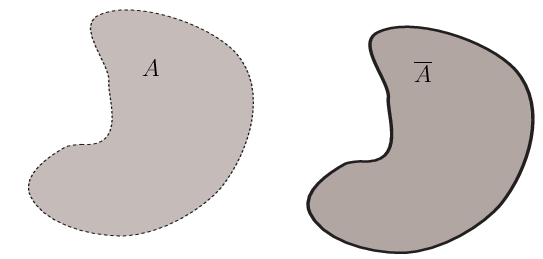
\includegraphics[scale=.5]{imagenes/clausu.png}
	\caption{Clausura de un conjunto}\label{fig,clausura}
\end{center}
\end{figure}

Tenemos la siguiente caracterización alternativa de clausura de
un conjunto.
\begin{proposicion}\label{pro,clausura} Sea $(X,d)$ un e.m. y $A\subset X$. Son
equivalentes:
\begin{itemize}
\item[a)] $x\in \C{A}$.
\item[b)] $\forall r>0: B(x,r)\cap A\neq\emptyset$.
\end{itemize}
\end{proposicion}
\begin{demo}Veamos primero que a)$\Rightarrow$b). Sea $x\in \C{A}$. Por
definición $x\notin (A^c)^0$. Así, por definición de
conjunto interior, tenemos que para todo $r>0$, $B(x,r)\nsubseteq
A^c$. Es decir que para todo $r>0$ existe $y=y_r\in B(x,r)\cap A$.
Esto prueba b).

Veamos ahora que b)$\Rightarrow$a). Sea, pues, $x$ un punto
satisfaciendo la propiedad b). Toda bola de radio $x$ y centro
$r>0$ corta al conjunto $A$. De modo que no existe una de tales
bolas con la propiedad que este completamente contenida en el
conjunto $A^c$. Esto nos dice, por definicion de conjunto
interior, que $x$ no está en el interior de $A^c$. Dicho de otro
modo $x\in \bigl[(A^c)^0\bigr]^c$.
\end{demo}

Las propiedades del interior tienen propiedades duales
correspondientes para la clausura.

\begin{teorema} Sean $(X,d)$ un e.m., $A$ y $B$ subconjuntos de
$X$. Entonces tenemos que:
\begin{itemize}
\item[a)] $A\subset \C{A}$.
\item[b)] El conjunto $\C{A}$ es el menor conjunto cerrado que
contiene a $A$.
\item[c)] $\C{\C{A}}=\C{A}$.
\item[d)] Si $A\subset B$ entonces $\C{A}\subset \C{B}$.
\item[e)]$\C{A\cup B}=\C{A}\cup \C{B}$.
\item[f)]$x\in \C{A}\Leftrightarrow d(x,A)=0$
\end{itemize}
\end{teorema}
\begin{demo} Veamos a) cuya propiedad dual es que $C^0\subset C$.
En efecto, tenemos que:

\[(A^c)^0\subset A^c.\]
Ahora, tomando complementos a ambos miembros\footnote{La
operación de complemento invierte las inclusiones}, obtenemos
que:
\[\C{A}=\bigl[(A^c)^0\bigr]^c\supset (A^c)^c=A.\]
Esto prueba a).

Veamos b). El conjunto $\C{A}$ es cerrado pues es el complemento
del abierto $(A^c)^0$. Sea $F$ un conjunto cerrado que contiene a
$A$, hay que demostrar que $F\supset \C{A}$. Entonces, tomando
complemento, tenemos que $F^c$ es un abierto contenido en $A^c$.
Como $(A^c)^0$ es el mayor abierto contenido en $A^c$, tenemos que
$F^c\subset (A^c)^0$. Ahora tomemos complemento a esta última
inclusión y obtenemos
\[F\supset \bigl[(A^c)^0\bigr]^c=\C{A},\]
que es lo que queríamos demostrar.

Como corolario de b), obtenemos que  $A$ es cerrado si, y solo si,
$\C{A}=A$. A su vez, como corolario de esto, obtemos c) y d).

Veamos e). Tenemos que:

\begin{align}
  \C{A\cup B}&=\bigl[(A\cup B)^c)^0\bigr]^c         &\qquad &\text{Definición clausura}\notag \\
			 &=\bigl[(A^c\cap B^c)^0\bigr]^c    &&\text{Leyes de de         Morgan}\notag\\
			 &=\bigl[(A^c)^0\cap (B^c)^0)\bigr]^c &&\text{Propiedad dual del interior}\notag\\
			 &=\bigl[(A^c)^0\bigr]^c\cup \bigl[(B^c)^0)\bigr]^c &&\text{Leyes de de Morgan}\notag\\
			 &= \C{A}\cup \C{B}                     &&\text{Definición de
			 clausura}\notag
  \end{align}


Que es lo que queríamos demostrar.

Por último demostremos f). Si $x\in \C{A}$ entonces, como
consecuancia de la proposición \vref{pro,clausura}, tenemos que
para todo $n\in\nn$ existe un $y_n\in A$ tal que $d(x,y_n)<1/n$,
ver figura \vref{fig,incf)}.


Tenemos asi que
\[d(x,A)=\inf\limits_{y\in A}d(x,y)\leq d(x,y_n)\leq \frac1n.\]
Y como la desigualdad es válida para todo $n\in\nn$, obtenemos
que $d(x,A)=0$.

Recíprocamente, si $d(x,A)=0$ entonces, por definición del
ínfimo, para todo $r>0$ existe un $y=y_r\in A$ tal que
$d(x,y)<r$. Así tenemos que $B(x,r)\cap A\neq \emptyset$,
para todo $r>0$. Esto, como sabemos, es equivalente a afirmar que
$x\in \C{A}$.
\end{demo}

Por último estamos interesados en definir aquellos puntos que
estan en lo que hemos denominado, sin ninguna precisión, borde
de un conjunto.

\begin{definicion} Diremos que $x$ pertenece a la \emph{frontera} de un
conjunto $A$ cuando $x$ está en la clausura de $A$ y en la
clausura de $A^c$. Llamamos al conjunto de todos los puntos
frontera de $A$ la \emph{frontera }de $A$ y denotaremnos este
conjunto por $\partial A$. \end{definicion}


La costumbre de denotar la frontera de un conjunto con el signo de
una derivada proviene, suponemos, del calculo sobre variedades
donde se observa que cierta integral de una ``derivada'' sobre un
conjunto es igual a la integral de la función sobre la frontera
del conjunto. Este resultado se conoce como Teorema de Stokes. El
Teorema fundamenteal del Cálculo es un caso particular de este
teorema. Es en este contexto donde se consigue una conexión
entre derivadas y fronteras.






\section{Ejercicios}

\begin{ejercicio}\label{ejmeteuclidea} Demostrar que los siguientes son espacios métricos.

\begin{itemize}
	\item[a)] $(\mathbb{R},d)$ donde $d$ está definida en
	\vref{distmod}.
	\item[b)]  $(\mathbb{R}^n, d)$ donde $d$ está definida en \vref{meteuclidea}.
	\emph{Ayuda:} Usar
la desigueladad de Cauchy-Schwartz
$\forall\mathbf{x}\in\mathbb{R}^n\forall\mathbf{y}\in\mathbb{R}^n$:
\[
	\sum\limits_{i=1}^{n}x_iy_i\leq
	\sqrt{\sum\limits_{i=1}^{n}|x_i|^2}
	\sqrt{\sum\limits_{i=1}^{n}|y_i|^2}
\]
\item[c)] $(\mathbb{R}^n, d)$, donde $d$ es la función definida
en \vref{l1met}.

\item[d)]$(\mathbb{R}^n, d)$, donde $d$ es la función definida
en \vref{linfmet}.
\item[e)] Probar que la métrica discreta es, valga la
redundancia, una métrica.
\item[f)] Demostrar que las ecuaciones \vref{convunifmet} y
\vref{l1metint} definen métricas.
\end{itemize}
\end{ejercicio}

\begin{ejercicio}\label{deslipschitz} Sea $(X,d)$ un espacio métrico. Demostrar que
para todos $x$ , $y$ y $z$ en $X$ tenemos que:
\[|d(x,y)-d(x,z)|\leq d(y,z).\]
\end{ejercicio}

\begin{ejercicio}\label{daconjeslipschitz} Sea $(X,d)$ un espacio
métrico y $A\subset X$. Demostrar que:
\[|d(x,A)-d(y,A)|\leq d(x,y).\]
\end{ejercicio}

\begin{ejercicio}\label{ejer,distequiv} Sea $(X,d)$ un e.m., probar que las siguientes
funciones son métricas sobre $X$:
\begin{itemize}
\item[a)] $d_1(x,y):=\min\{1,d(x,y)\}$.
\item[b)] $d_2(x,y):=\frac{d(x,y)}{1+d(x,y)}$.
\end{itemize}
\end{ejercicio}

\begin{ejercicio} Sea $(X,d)$ un e.m.. Demostrar que $\forall
x,y\in X$, existe entornos $U\in E(x)$ y $V\in E(y)$ tales que
$U\cap V=\emptyset$.
\end{ejercicio}

\begin{ejercicio} Sea $(X,d)$ u e.m.. Demostrar las siguientes
propiedades:
\begin{itemize}
	\item[a)] Si $A\subset X$ es finito, entonces $X-A$ es abierto.
	\item[b)] Si $A\subset X$ es abierto, entonces para todo
	conjunto $B$ se tiene que $A\cap \C{B}\subset \C{A\cap B}$.
	\item[c)] Si $A$ es abierto entonces $A\subset (\C{A})^0$.
	\item[d)] Si $A$ es cerrado entonces $(\C{A})^0\subset A$.
	\item[e)]
	$(\C{A})^0=\C{\biggl(\C{\bigl((\C{A})^0\bigr)}\biggr)}$.
	\item[f)]
	$\C{(A^0)}=\C{\biggl(\C{\bigl(\C{(A^0)}\bigr)^0}\biggr)}$.
	\item[g)] $A^0=\bigl(\C{A^c}\bigr)^c$.
	\item[h)] $\partial A=\C{A}-A^0$.
	\item[i)] $\text{Ext}(A)=(\C{A})^c$.
	\item[j)] $\partial A^0\subset \partial A$ y $\partial
	\C{A}\subset \partial A$.
	\item[k)] $\partial (A\cup B)\subset \partial A\cup\partial
	B$, Si $\C{A}\cap\C{B}=\emptyset$ entonces vale la igualdad en
	la anterior inclusión.
	\item[l)] $d(A,B)=d(\C{A},\C{B})$, donde por definición:
	\[
		d(A,B):=\inf\limits_{x\in A,y\in B}d(x,y).
	\]
\end{itemize}
\end{ejercicio}
\begin{ejercicio} Dar ejemplos de:
\begin{itemize}
\item[a)] $A$ y $B$ abiertos de $\rr$ tales que los siguientes
conjuntos sean todos diferentes: $\C{A}\cap \C{B}$, $\C{A\cap B}$,
$\C{A}\cap B$, $A\cap \C{B}$.
\item[b)] $A$ y $B$ intervalos de $\rr$ tales que
$A\cap\C{B}\nsubseteq \C{A\cap B}$.
\item[c)] $A\subset \rr^2$ tal que $\partial A=A$.
\item[d)] $A$ y $B$ subconjuntos de $\rr^2$ tales que entre los
siguientes conjuntos no valga ninguna inclusión: $\partial
A\cup\partial B-\partial(A\cap B)$ y $\partial (A\cup B)$.
\end{itemize}
\end{ejercicio}
\begin{ejercicio} Demostrar que los siguientes conjuntos de
$\rr^2$ y $\rr^3$, son abiertos con la métrica euclidea:
\begin{itemize}
\item[a)] $\{(x,y)\in\rr^2: m<d\bigl((x,y),(0,0)\bigr)<n\}$, donde
$n,m\in\nn$ y $m<n$.
\item[b)] $\{(x,y)\in\rr^2: 0<x<1,\,\, 0<y<1,\,\,x\neq
\frac1n\,\,\forall n\in\nn\}$.
\item[c)] $\{(x,y,z)\in\rr^3: x,y,z\in\mathbb{Z}\}^c$.
\end{itemize}
\end{ejercicio}
\begin{ejercicio} Hallar la frontera y el diámetro del conjunto
$\{\frac1n:n\in\nn\}$.
\end{ejercicio}
\begin{ejercicio} Demostrar que el diámetro de la dola unitaria
en $\rr^2$ con la métrica euclidea es 2.
\end{ejercicio}
\begin{ejercicio} Un e.m. $(X,d)$ se dice ultramétrico si $d$ verifica la
desigualdad ultramétrica, es decir:
\[
	d(x,y)\leq\max\{d(x,z),d(z,y)\}.
\]
Sea $X$ un e.m. ultramétrico. Demostrar que:
\begin{itemize}
\item[a)] Si $d(x,y)\neq d(y,z)$ entonces
$d(x,z)=\max\{d(x,y),d(y,z)\}$.
\item[b)] Si $y\in B(x,r)$ entonces $B(x,r)=B(y,r)$. Como
consecuencia las bolas abiertas son también conjuntos cerrados.
\item[c)] Si $y\in\C{B(x,r)}$ entonces $\C{B(y,r)}=\C{B(x,r)}$.
Las bolas cerradas son, también, conjuntos abiertos.

\item[d)] Si dos bolas tienen intersección no vacía
entonces una está  contenidad en la otra.

\item[e)] La distancia de dos bolas abiertas distintas de radio
$r$, contenidas en una bola cerrada de radio $r$, es igual a $r$.
\end{itemize}
\end{ejercicio}
